\documentclass[10pt,a4paper]{article}
\usepackage[margin=16mm]{geometry}
\usepackage{graphicx}
\usepackage{booktabs}
\usepackage{array}
\usepackage{enumitem}
\usepackage[hidelinks]{hyperref}
\setlength{\parskip}{3pt}
\setlength{\parindent}{0pt}
\renewcommand{\arraystretch}{1.12}
\newcommand{\code}[1]{\texttt{#1}}

\begin{document}

\begin{center}
{\Large Digital VLSI Assignment: 4-bit Array Multiplier from RTL to GDSII}\\[3pt]
{\large Jainil Bavishi \quad|\quad Roll No. 2023102045}\\[2pt]
SkyWater SKY130 \code{sky130\_fd\_sc\_hd} standard-cell library
\end{center}

\section{Introduction}
This report implements a registered, unsigned 4-bit by 4-bit array multiplier and takes it from structural Verilog to a routed GDSII layout. The flow used Icarus Verilog for simulation, Yosys for synthesis, OpenSTA for timing analysis, and LibreLane for physical design. All generated artifacts, scripts, logs and the final GDSII are included in the repository.

\section{Design and verification (Part A)}
The multiplier registers \code{a[3:0]} and \code{b[3:0]}, forms four partial-product rows, and adds rows 1--3 with exactly 12 instances of \code{full\_adder}. Row 0 contributes \code{p[0]}; the final combinational result is captured in the 8-bit output register. There are therefore 16 AND gates, 12 full adders and 16 flip-flops. An input applied before edge 1 is captured at edge 1 and its product is captured at edge 2, giving a latency of 2 cycles and a throughput of 1 result per cycle.

\begin{figure}[h]
\centering
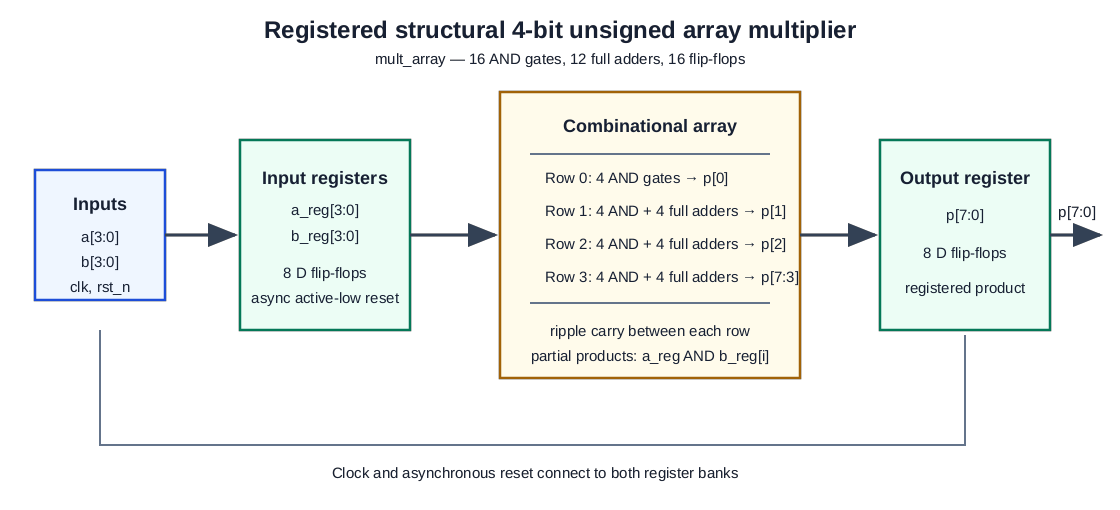
\includegraphics[width=0.94\linewidth]{array_multiplier_block.png}
\caption{Structural organization of the registered 4-bit array multiplier.}
\end{figure}

The self-checking testbench holds asynchronous reset low for the first 2 clock cycles, applies all 256 input pairs, waits for the 2-cycle latency, and compares the registered result with the reference value. RTL simulation reported \code{PASS: 256 vectors checked, 0 errors}; the synthesized gate-level netlist reported the same PASS line. To prove the checker detects errors, \code{sum = a \^{} b \^{} cin} was temporarily changed to \code{sum = a \^{} b}; the test then reported \code{FAIL: 256 vectors checked, 95 errors}, after which the correct RTL was restored.

For the required personal example, the last roll-number digit is 5, so $A=5+5=10$ and $B=7$. The hand calculation is $1010_2\times0111_2=1000110_2=70_{10}$.
\begin{verbatim}
      1010       (10)
    x 0111       (7)
    ------
      1010
     10100
    101000
   0000000
    ------
   1000110       (70)
\end{verbatim}
\begin{figure}[h]
\centering
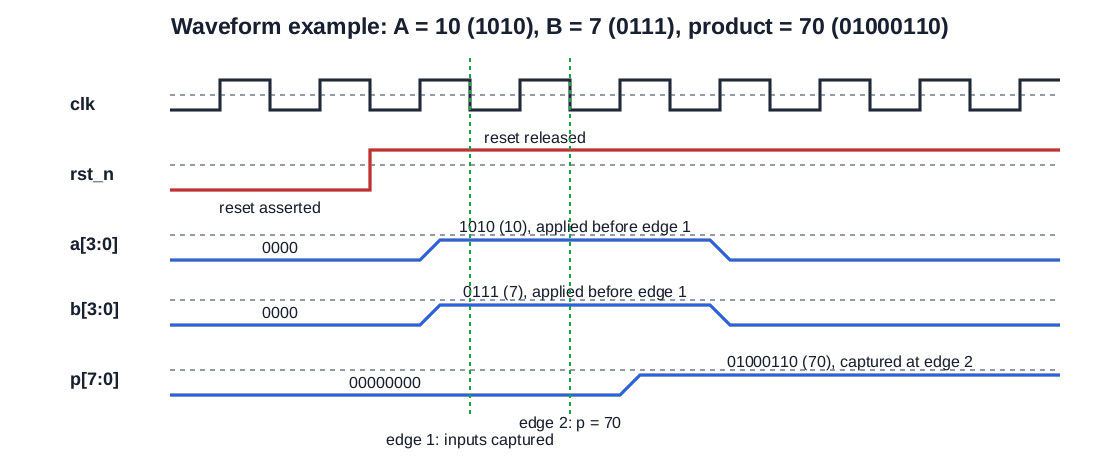
\includegraphics[width=0.96\linewidth]{waveform_example.png}
\caption{Waveform example for $A=10$ and $B=7$: the operands are captured at edge 1 and \code{p=70} is captured at edge 2.}
\end{figure}

\section{Synthesis (Part B)}
Yosys flattened the hierarchy, mapped registers with \code{dfflibmap}, mapped combinational logic with \code{abc}, and wrote the SKY130 gate-level netlist. Table~\ref{tab:synth} is taken from \code{synth/mult\_array\_stat.rpt}.

\begin{table}[h]
\centering\small
\caption{Yosys synthesis results in the SKY130 standard-cell library.}\label{tab:synth}
\begin{tabular}{@{}lr@{}}
\toprule
Metric & Measured value \\
\midrule
Total number of cells & 63 cells \\
Flip-flops & 16 \code{sky130\_fd\_sc\_hd\_\_dfrtp\_1} cells \\
Total cell area & 740.7104 $\mu$m$^2$ \\
Flip-flop area & 400.3840 $\mu$m$^2$ \\
Flip-flop share & 54.05\% \\
Most-used cell types & \code{dfrtp\_1}: 16; \code{nand2\_1}: 8; \code{a21oi\_1}: 6 \\
Gate-level exhaustive simulation & PASS: 256 vectors checked, 0 errors \\
\bottomrule
\end{tabular}
\end{table}

There are $63-16=47$ mapped logic cells. This is not simply $16+12=28$ because a full-adder Boolean function is decomposed into several available library gates, and the mapper optimizes and buffers the complete flattened network.

\section{Static timing analysis (Part C)}
OpenSTA used the typical \code{tt\_025C\_1v80} Liberty corner, a 1.00 ns input delay and a 1.00 ns output delay. At the required initial 10.00 ns period, the reported worst setup slack was 7.40 ns; applying the assignment formula gives $T_{min}=10.00-7.40=2.60$ ns and $F_{max}=1000/2.60=384.615$ MHz. Re-running at 2.60 ns gave $-0.004$ ns setup slack, which is close to zero after the required 0.01 ns rounding.

\begin{table}[h]
\centering\small
\caption{OpenSTA maximum-delay timing results.}\label{tab:sta}
\begin{tabular}{@{}lr@{}}
\toprule
Metric & Measured value \\
\midrule
Worst slack at 10.00 ns & 7.40 ns \\
$T_{min}$ & 2.60 ns \\
$F_{max}$ & 384.615 MHz \\
Slack at $T_{min}$ & $-0.004$ ns \\
Critical-path start point & \code{\_095\_/Q} (input register) \\
Critical-path end point & \code{\_092\_/D} (output register) \\
Cells on the path & 10 cells including the two endpoint flip-flops \\
Latency $=2T_{min}$ & 5.20 ns \\
Throughput & 384.615 million results/s \\
\bottomrule
\end{tabular}
\end{table}

The path order is \code{dfrtp\_1}, \code{clkinv\_1}, \code{o311ai\_0}, \code{a21oi\_1}, \code{maj3\_1}, \code{xnor2\_1}, \code{maj3\_1}, \code{maj3\_1}, \code{xnor3\_1}, \code{dfrtp\_1}. Thus it has 8 mapped combinational cells between the launch and capture registers. These gates are the mapped form of the carry/sum logic, rather than one library cell per full adder; the path follows the expected ripple-carry part of the array and is consistent with the approximately $2N=8$ full-adder-delay estimate for $N=4$.

\section{Physical design (Part D)}
The required first LibreLane period from $1.2T_{min}$ is 3.50 ns. Setup timing was negative at 3.50, 4.00, 4.50, 5.00, 5.50 and 6.00 ns, so the period was increased by 0.50 ns each run. The seventh run at 6.50 ns completed with non-negative setup slack, 0 Magic DRC errors and 0 LVS errors. The submitted \code{metrics.json} and \code{mult\_array.gds} are copied from that successful final run.

\begin{table}[h]
\centering\small
\caption{Final LibreLane physical-design results at a 6.50 ns clock period.}\label{tab:pnr}
\begin{tabular}{@{}lr@{}}
\toprule
Metric & Measured value \\
\midrule
CLOCK\_PERIOD / successful runs & 6.50 ns / 7 runs \\
Core area / die area & 17,759.5 $\mu$m$^2$ / 22,500 $\mu$m$^2$ \\
Cells after synthesis / place and route & 63 cells / 1,901 instances \\
Added cell kinds & 1,566 fillers; 245 taps; 19 repair buffers; 3 clock buffers \\
Routed wirelength & 2,405 $\mu$m \\
Worst setup slack & 0.0853 ns \\
Post-route $F_{max}$ & 155.891 MHz \\
Part C $F_{max}$ & 384.615 MHz \\
Magic DRC errors / LVS errors & 0 errors / 0 errors \\
\bottomrule
\end{tabular}
\end{table}

\begin{figure}[h]
\centering
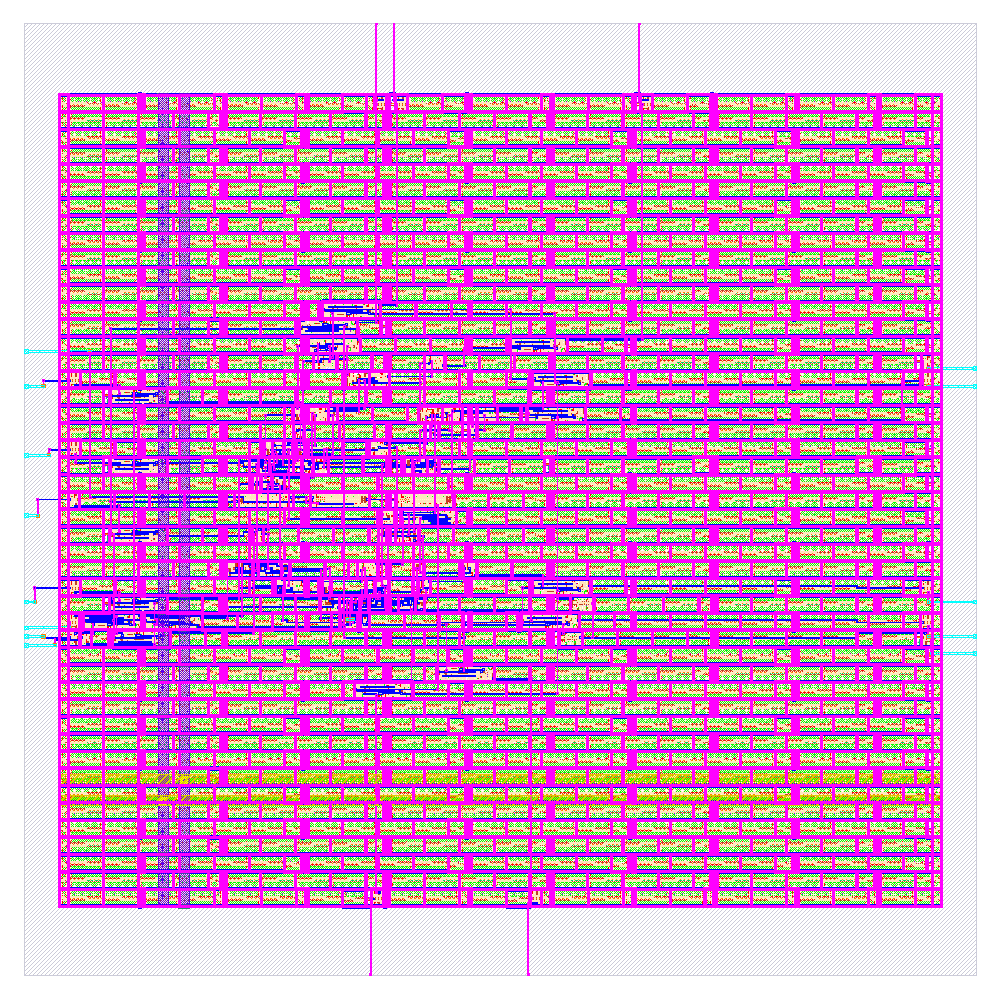
\includegraphics[width=0.52\linewidth]{layout_whole_die.png}
\caption{Final 150 $\mu$m by 150 $\mu$m GDSII layout, whole-die view.}
\end{figure}
\begin{figure}[h]
\centering
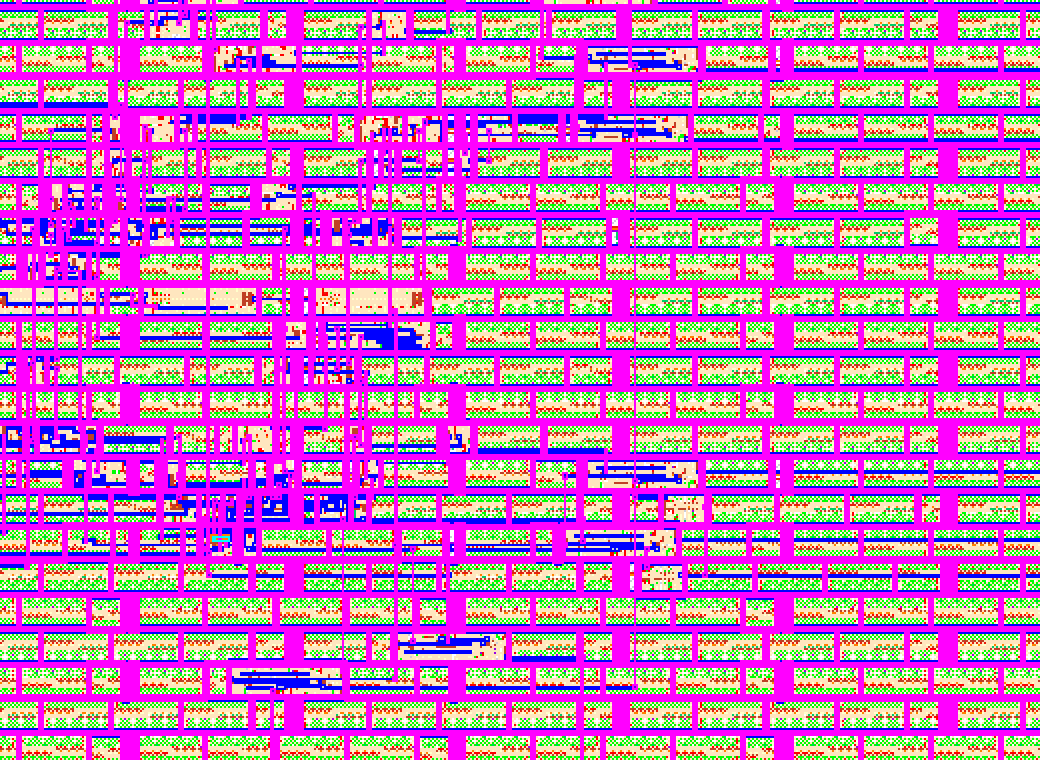
\includegraphics[width=0.80\linewidth]{layout_zoomed.png}
\caption{Close-up of the final layout showing standard-cell rows and routed metal.}
\end{figure}

\section{Answers to questions}
\begin{enumerate}[leftmargin=*,label=\textbf{\arabic*.}]
\item Synthesis produced 47 logic cells after subtracting the 16 flip-flops from the 63-cell total. The structural count of 16 AND gates plus 12 full adders counts RTL blocks, whereas the standard-cell library implements each full adder with several Boolean gates and the mapper also optimizes, inverts and buffers the flattened logic.
\item The critical path runs from input-register output \code{\_095\_/Q} to output-register input \code{\_092\_/D}. It contains 10 library cells including its two flip-flop endpoints, or 8 combinational mapped cells. The sequence passes through carry/sum logic represented by AOI, majority and XNOR gates; this is consistent with the approximate 8 full-adder-delay ripple estimate, although technology mapping does not preserve a one-cell-per-full-adder correspondence.
\item Flip-flops occupy $400.3840/740.7104\times100=54.05\%$ of the synthesized cell area. This is large because the design has a fixed 16-register overhead, while a 4-bit multiplier contains a small amount of combinational logic; the input and output registers together are wider than either operand.
\item The post-route frequency of 155.891 MHz is lower than the 384.615 MHz pre-layout result because routing adds wire resistance/capacitance, clock-tree delay and signoff corner constraints. LibreLane added 1,566 filler cells to fill legal rows, 245 tap cells for substrate/well connections, 19 repair buffers for timing/electrical repair, and 3 clock buffers to distribute the clock.
\item DRC checks whether the drawn layout obeys process geometry rules such as widths, spacing and enclosure. LVS compares the extracted layout connectivity with the intended netlist. Both must pass: a layout can meet geometric rules but connect the wrong nets, or connect the right nets while violating manufacturing rules.
\item For an $N$-bit array, the number of AND gates is $N^2$ and the number of full adders is $N(N-1)$. At $N=8$, this gives $8^2=64$ AND gates and $8(8-1)=56$ full adders, compared with 16 and 12 at $N=4$. The path estimate changes from $2\times4=8$ to $2\times8=16$ full-adder delays, so the delay is roughly doubled and the maximum frequency is roughly halved before layout effects.
\end{enumerate}

\section{Conclusion}
The structural RTL, exhaustive RTL simulation, deliberate fault-injection check, synthesized netlist simulation, OpenSTA timing analysis and LibreLane implementation were completed. The final 6.50 ns layout has positive setup slack, 0 Magic DRC errors and 0 LVS errors; the final GDSII and all reproducibility scripts are included with this report.

\end{document}
